\chapter{How to use this template}

\section{First Section}

Uses kpfonts.

\begin{defn}[Definition Title]{label_defn1}
	A definition. The title is optional.
\end{defn}



\begin{exmpl}[Title]{label_exmpl}
	\begin{itemize}
		\item First example 
		\begin{itemize}
			\item  Note $1$
			\item  Note $2$
		\end{itemize}
		\item Second example
	\end{itemize}
\end{exmpl}    



Some other text.

\begin{theo}[Theorem Title]{label_thm}
	A Theorem that uses objects defined in \cref{label_defn1}. Title is optional. 
	\[\dint_a^b u v' \dx = [u(x)v(x)] \eval_a^b - \dint_a^b u'(x) v(x) \dx\]
\end{theo}


\begin{prf}{label_thm}
	Proof text ends in qed symbol. Must be supplied the label of the theorem.
\end{prf}


\begin{exercise}[Questions have their own counters.]\label{question_label}
	\begin{enumerate}
		\item Greek letters and uppercase math letters are always upright. Such as \label{step_a}
		\begin{enumerate}
			\item  $\alpha x^2 +\beta$ \label{substep_a_i} 
			\item  $y =mx+ C \in \R$ 
		\end{enumerate}
		
		\item Do the  following tasks after \ref{step_a}.
		\begin{tasks}(3)
			\task first do \ref{substep_a_i}.
			\task ??    
			\task Profit
		\end{tasks}
\end{enumerate}
\end{exercise}

\begin{solution}
	Solution to the exercise. Uncomment the ``solutionfalse'' flag to make solutions invisible.
\end{solution}


\begin{note}[Fun Fact:]
	This is a note with a custom title. Default is `Note:'.
\end{note}



\section{Second Section}

Let's start with a picture that explains the main idea:
\begin{figure}[!ht]
    \centering
    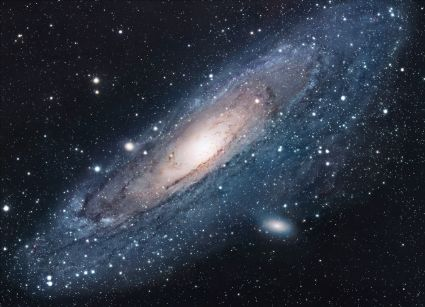
\includegraphics[width=0.5\textwidth]{images/universe.jpg}
    \caption{The Universe}
    \label{fig:universe}
\end{figure}


\begin{axiom}{label_axiom}
	This is an axiom.
\end{axiom}

\begin{prop}{label_proposition}
	This is a proposition.
\end{prop}

\begin{claim}{label_claim}
	This is a claim.
\end{claim}

\begin{digression}
	A digression into tangentially related topics.
\end{digression}



\subsection{Case 1: First subsection}
When  \cref{label_exmpl} is true.
\begin{warning}[A Warning:] %default is Warning:
	\lipsum[1][1-2]
\end{warning}

\subsection{Case 2: Second subsection}
Do \cref{question_label} first.

Computer Code is written as {\tt Typewriter font}.

\begin{code}{Python}
    def rk4(f,x0,t0,tmax,dt):
        t = # build the time array
        x = # initialize an empty array for the x values
        x[0] = # build the initial condition
        # On the next line: be careful about how far you're looping
        for i in range( ??? ):
        # The interesting part of the code goes here.
        # Start from t[i] and x[i]. Then Define k1, k2, k3, k4 
        # and use them to find x[i+1]
        return t, x
        
    f = lambda t, x: # the definition of the function goes here
    
    x0 = # initial condition
    t0 = 0
    tmax = # your choice
    dt = # pick something reasonable
    t, x = rk4( ??? , ??? , ??? , ??? , ??? )
    # plot t vs. x
\end{code}
